%\documentstyle[epsf,twocolumn]{jarticle}       %LaTeX2.09仕様
\documentclass[twocolumn]{jarticle}     %pLaTeX2e仕様

%\usepackage[backend=bibtex, style=numeric]{biblatex}
%\addbibresource{sankou.bib}
%%%%%%%%%%%%%%%%%%%%%%%%%%%%%%%%%%%%%%%%%%%%%%%%%%%%%%%%%%%%%%
%%
%%  基本 バージョン
%%
%%%%%%%%%%%%%%%%%%%%%%%%%%%%%%%%%%%%%%%%%%%%%%%%%%%%%%%%%%%%%%%%
\setlength{\topmargin}{-45pt}
%\setlength{\oddsidemargin}{0cm}
\setlength{\oddsidemargin}{-7.5mm}
%\setlength{\evensidemargin}{0cm}
\setlength{\textheight}{24.1cm}
%setlength{\textheight}{25cm}
\setlength{\textwidth}{17.4cm}
%\setlength{\textwidth}{172mm}
\setlength{\columnsep}{11mm}

\setlength{\intextsep}{8pt}
\setlength{\textfloatsep}{8pt}
\setlength{\floatsep}{1pt}

\kanjiskip=.07zw plus.5pt minus.5pt



%【節がかわるごとに(1.1)(1.2) …(2.1)(2.2)と数式番号をつけるとき】
%\makeatletter
%\renewcommand{\theequation}{%
%\thesection.\arabic{equation}} %\@addtoreset{equation}{section}
%\makeatother

%\renewcommand{\arraystretch}{0.95} 行間の設定

\usepackage[dvipdfmx]{graphicx}   %pLaTeX2e仕様(\documentstyle ->\documentclass)
\usepackage[dvipdfmx]{color}
\usepackage{scalefnt}
\usepackage{bm}
\usepackage{here}
\usepackage{url}
\usepackage{amsmath}
\usepackage{siunitx}
\usepackage{amsfonts}
\usepackage[subrefformat=parens]{subcaption}
\captionsetup{compatibility=false}
%%%%%%%%%%%%%%%%%%%%%%%%%%%%%%%%%%%%%%%%%%%%%%%%%%%%%%%%
\usepackage{comment}
\usepackage{subcaption}
\usepackage{multirow}
\usepackage{nidanfloat}
%\usepackage[table,xcdraw]{xcolor}
\usepackage[dvipdfmx]{hyperref}
\usepackage{caption}
\usepackage[normalem]{ulem}
\useunder{\uline}{\ul}{}

\begin{document}

\twocolumn[
\noindent
\hspace{1em}

前期研究発表会資料 令和 3 年 6 月 14 日 (月)
\hfill
\ \ M1 高山 裕成

\vspace{2mm}
\hrule
\begin{center}
{\Large  深層学習によるマルチメディアデータを入力とした動作ラベルの推定}
\end{center}
\hrule
\vspace{3mm}
]

\section{はじめに}
近年, 深層学習を始めとする機械学習技術の大きな発展を受けて, 人工知能を用いた創作物理解が注目されている.
しかし, 創作は高次の知的活動であるため, いまだに実現が困難なタスクである.
人の創作物の理解に関する分野の中でも動画を対象とした研究は,
画像データ, 音声データ, テキストデータといったマルチメディアデータを扱う分野である. 動画を対象とした生成タスクの例は, 白黒映像に色情報を付与する自動着色や, 映像を滑らかにするフレーム補間, 動画に対する音声の自動生成などがあり, 活発な研究分野である. 本研究では, 最終目標を深層学習によるマルチメディアデータを用いた動画に対する音声の自動アノテーションモデルの構築とし, 本稿では前段階である, 動画に含まれるマルチメディアデータから動画の動作を推定する手法について述べる.

\section{関連研究}
動画に対する音声の自動生成に関連した研究として, Yipin らの研究 \cite{DBLP:journals/corr/abs-1712-01393} について述べる. Yipin らは, 図 \ref{fig:visual_ex} に示すように音声の生成部分に RNN を階層状に積み, 上層ほど長い間隔の依存をとらえるのを担当するような構成を構築した SampleRNN を用いて, SampleRNN の最上階層への入力として, 学習済みの VGG19 モデルを用いてフレーム画像から得た特徴量や, 入力映像の内容と動きをより捉えるために, オプティカルフローを使用することで高精度な音声の生成を可能にした.

\begin{figure}[bht]
  \centering
  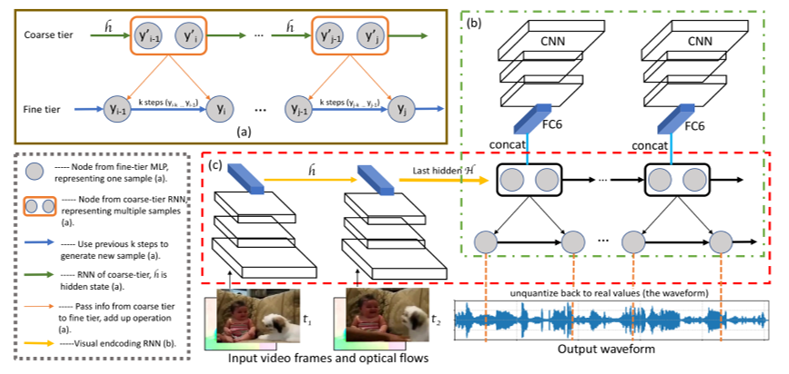
\includegraphics[scale=0.34]{visual_ex.png}
  \caption{文献 \cite{DBLP:journals/corr/abs-1712-01393} における音声生成モデル}
  \label{fig:visual_ex}
\end{figure}

\section{データセット}
動画に関係したデータセットには, Kinetics や Moments in Time などがあるが, 本研究では STAIR Actions \cite{yoshikawa2018stair} を用いた. これは, STAIR Lab らによって作成された家庭内で見られる人間の行動 100 種類を集めた行動認識研究のための大規模な動画データセットである. STAIR Actions データセットに含まれる動画の半数は Youtube から取得された動画, 残りの半数はクラウドソーシングによって作成された動画から構成されており, 1 つの動画には 1 つの動作ラベルが付与されている. さらに, クラウドソーシングによって 1 つの動画につき平均 5 つの検品済み日本語キャプションがアノテートされており,「誰が」(Who),「どこで」(place),「何をしているか」(action) の情報が含まれている.


\section{要素技術}
\subsection{メル尺度, メルスペクトログラム}
メル尺度とは音高の知覚的尺度の一つで, 人間が高い周波数よりも低い周波数の違いを検出するのが得意である特性に合わせてメル尺度の差が同じであれば, 人間が感じる音高の差が同じになるようにスケール変換したものである. メル尺度と通常の周波数測定値との基準点として, $1000 \si{\hertz}$ の音が $1000$ メル ($mels$) の音高と定義されており, 周波数 $f$ をメル尺度 $m$ に変換する一般式は,
\begin{equation}
  m = m_{0}\ln(\frac{f}{f_{0}}+1)
\end{equation}
で表される. ここで, $f_{0}$ は自由な周波数パラメータで, $m_{0}$ は 定義から導かれる式,
\begin{equation}
  m_{0} = \frac{1000}{\ln(\frac{1000}{f_{0}} + 1)}
\end{equation}
から算出される従属パラメータである. そして, 信号を短時間フーリエ変換して得られたスペクトログラムに対して, 周波数をこのメル尺度に変換したものをメルスペクトログラムという.

\newpage
\subsection{SpecAugment}
SpecAugment \cite{Park_2019} とは, 2019 年に Google Brain が提案した音声データの拡張手法であり, 3 つの変換方式
\begin{itemize}
  \item Time Warping
  \item Frequency Masking
  \item Time Masking
\end{itemize}
から構成されている. Time Warping は, スペクトログラムに対してランダムに選んだ点を時間軸方向に動かし, 動かした分だけ点の左右に存在する矩形領域を伸び縮みさせ, 時間方向の変調を行う. Frequency Masking は数チャネル分の周波数成分をマスキングし, Time Masking は数ステップ分の時間軸成分をマスキングする.
本研究では, Frequency Masking および Time Masking のみを扱う. 図 \ref{fig:spec_aug} にメルスペクトログラムに対して Frequency Masking と Time Masking を適応した例を示す.

\begin{figure}[tb]
  \centering
  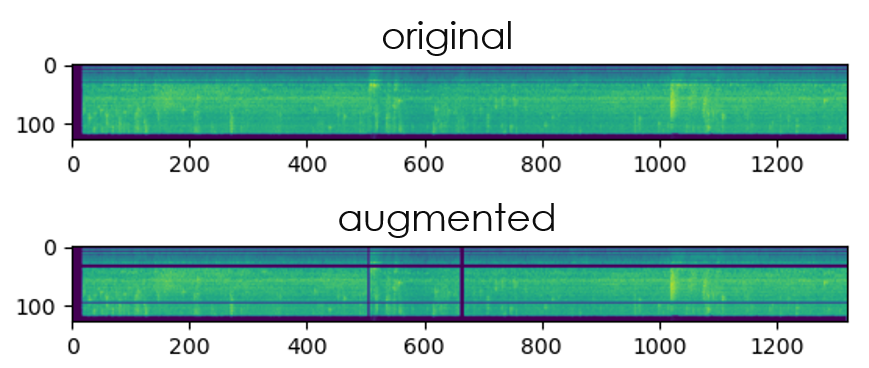
\includegraphics[scale=0.5]{spec_aug.png}
  \caption{SpecAugment 例}
  \label{fig:spec_aug}
\end{figure}


% \subsection{VGG}
% VGG \cite{brusilovsky:simonyan2014very} とは, ImageNet と呼ばれる大規模
% 画像データセットで学習済みの畳み込みニューラルネットワークであり, 構成する層の数に応じて VGG11 や VGG16 などと呼ばれている.
% % VGG16 : 13 層の畳み込み層と 3 層の全結合層の合計 16 層からなる

\subsection{Residual Network (ResNet)}
Residual Network (ResNet) \cite{DBLP:journals/corr/HeZRS15} は Microsoft Research が 2015 年に考案した手法である. ショートカット接続機構を導入し, 手前の層の入力を後ろの層に直接足し合わせることで, ある層で求める最適な出力を学習するのではなく, 層の入力を参照した残差関数を学習し, 勾配消失問題を解決した.

\subsection{Word2Vec, Doc2Vec}
Word2Vec \cite{word2vec} は単語の分散表現を獲得する手法の 1 つである.
この手法は,同じ文脈で出現する単語は類似した意味を持つと予想されることに基づいており,
写像されたベクトルは, One-hot 表現のような局所表現と異なり, 単語間の意味を考慮した類似度測定や, $「王様」-「男」+「女」=「女王」$のような単語間の意味における演算などができるようになる.
Word2Vec では, 自己から周りの単語あるいは周りの単語から自己を予測することにより分散表現を獲得する.
前者の手法を Skip-gram といい, 後者の手法を Countinuous Bag-of-Words (CBOW) という.

Doc2Vec \cite{DBLP:journals/corr/LeM14} は Word2Vec をベースとした, 文書をベクトル空間上に写像し
て分散表現を得る自然言語処理の手法である.
Paragraph ID は各文書と紐づいており, 単語の学習時に一緒にこの Paragraph ID を学習することで文書の分散表現を獲得する.
このベクトルを用いると文書間の類似度の算出や文書間での加減算が可能になる.
CBOW を拡張したモデルを Distributed Memory モデルといい, Skip-gram を拡張したモデルを Distributed Bag-of-Words という.

\section{数値実験}
本研究では, STAIR Actions データセットの内, 動作ラベルが
``drinking", ``eating meal", ``washing face", ``gardening", ``fighting" の全 5 種類のみを用いて, 入力を動画に含まれる音声データまたはキャプションデータ, 出力を動作ラベルとする 5 クラス分類問題を学習した.

実験 1 および実験 2 では, 使用するデータからランダムで 50\% と 30\% サンプリングしたものをそれぞれ訓練用データおよび検証用データとし, 残り 20\% を評価用データとした. 損失関数に使うクラス重みとして訓練用データの各動作ラベルのデータ数の逆数を正規化したものを用いた. また, 検証用データにおける正解率 (以下, Acc と表記する) が最大となるエポックのモデルを評価用モデルとして採用し, モデルの性能を測った. このとき, ベースラインとしてはすべてをランダムに予測した場合とした.

\subsection{\small{実験 1: 音声を入力とする動作ラベル推定}}
音声データの前処理として, 学習の際には入力される時間長を合わせる必要があるため, 本研究では開始 $0$ 秒から $5$ 秒間のデータを切り出し, 長さが不足している場合は音声データを繰り返すことでパディングした. 次に, 音声データをメルスペクトログラムに変換し, 最後に次元数を $(2 \times 128 \times 128)$ にリサイズしたものをネットワークへの入力とした. ネットワークには VGG16 に Batch Normalization を導入した VGG16-BN と, ResNet34 の事前学習済みモデルを用いて最後の全結合層のみを fine tuning した. このとき, 音声データの入力次元とクラス数に合わせてアーキテクチャを一部変更している.
そして, 訓練用データに対して入力の度に SpecAugment を行う場合と行わない場合の 2 つの設定について学習し, 評価用データを用いて精度の結果を比較した.

表 \ref{table:audio_data_size} に実験 1 で用いたデータ数および動作ラベルごとの平均時間長, 表 \ref{table:ex_para} に学習時のパラメータ, 表 \ref{table:spec_aug_para} に SpecAugment のパラメータを示す.
実験 1 ではクラウドソーシングによって作成された動画データとその音声データのみを用いた.

表 \ref{table:res_ex1} に実験 1 の結果を示す. 表 \ref{table:res_ex1} より, どの場合もベースラインを超え, ネットワークに VGG16-BN を用いて SpecAugment をした時, 最も評価指標の値が高かった. 図 \ref{fig:resnet34_ex1} にネットワークに ResNet34 を用いた場合の学習曲線を示す. 図 \ref{fig:resnet34_ex1} より, SpecAugment をしたことで訓練用データの Acc が検証用データの Acc を下回るように学習が進んでいる一方で, 検証用データにおける loss の増加が抑えられており, ネットワークに VGG16-BN を用いた場合でも同じ傾向が見られた. この事より, SpecAugment によって過学習が抑えられ汎化性能が向上していると推測できるものの, 本実験で用いたハイパーパラメータは恣意的なものであるため, 妥当性が考慮されていない. よって optuna などを用いたハイパーパラメータのチューニングによって, 最大性能同士の比較が必要であると考えられる. 図 \ref{fig:ex1_cm_vgg} に SpecAugment を行わなかった場合の VGG16-BN における評価用データに対する混合行列を示す. 図 \ref{fig:ex1_cm_vgg} より, 5 つの動作ラベルの内, 精度が低かったのは ``drinking", ``eating meal" であり, どの実験設定でも同じ傾向が見られた. この原因としては, これら 2 つの動作ラベルが飲食に関わるものであることや, 動作そのものに音があまり伴わないデータが多かった事が挙げられる. その他にも動作ラベルに対応する前景よりも別動作に対応する背景の音声が強調されたものや無音であるデータも含まれていたため, データの選び方についても考慮すべき問題である.

\captionsetup[table]{font=footnotesize}
\captionsetup[table]{labelfont=footnotesize}

\begin{table*}[!thbp]
\begin{tabular}{cc}
\begin{minipage}[c]{0.5\hsize}
\centering
\caption{音声データ数}
\label{table:audio_data_size}
\scalebox{0.7}{
\begin{tabular}{l|ccc|c}
label & train & validation & test & avg length [sec] \\ \hline
drinking & 254 & 149 & 107 & $5.64 \pm 0.60$ \\
eating meal & 231 & 122 & 88 & $5.82 \pm 0.78$ \\
washing face & 490 & 308 & 177 & $5.59 \pm 0.68$ \\
gardening & 64 & 43 & 35 & $5.59 \pm 0.38$ \\
fighting & 130 & 81 & 61 & $5.64 \pm 0.32$ \\ \hline
合計 & 1169 (50\%) & 703 (30\%) & 468 (20\%) &
\end{tabular}
}
\end{minipage} &
\begin{minipage}[c]{0.5\hsize}
\centering
\caption{キャプションデータ数}
\label{table:caption_data_size}
\scalebox{0.7}{
\begin{tabular}{l|ccc}
label & train & validation & test \\ \hline
drinking & 646 & 390 & 268 \\
eating meal & 602 & 345 & 256 \\
washing face & 252 & 143 & 82 \\
gardening & 1005 & 623 & 416 \\
fighting & 1042 & 628 & 398 \\ \hline
合計 & 3547 (50\%) & 2129 (30\%) & 1420 (20\%)
\end{tabular}
}
\end{minipage}
\end {tabular}
\end{table*}

\begin{table}[!tbhp]
\begin{tabular}{cc}
\begin{minipage}[c]{0.5\hsize}
\centering
\caption{実験 1 結果}
\label{table:res_ex1}
\scalebox{0.7}{
\begin{tabular}{c|cc}
\multicolumn{1}{l|}{\multirow{2}{*}{}} & \multicolumn{2}{c}{評価指標} \\
\multicolumn{1}{l|}{} & Acc & \begin{tabular}[c]{@{}c@{}}F 値\\ (macro)\end{tabular} \\ \hline
VGG16-BN & 0.771 & 0.752 \\
\begin{tabular}[c]{@{}c@{}}VGG16-BN\\ \small{(SpecAugment)}\end{tabular} & {\ul 0.773} & {\ul 0.754} \\ \hline
ResNet34 & 0.756 & 0.740 \\
\begin{tabular}[c]{@{}c@{}}ResNet34\\ \small{(SpecAugment)}\end{tabular} & 0.741 & 0.724 \\ \hline
baseline & 0.200 & -
\end{tabular}
}
\end{minipage} &
\begin{minipage}[c]{0.5\hsize}
\centering
\caption{実験 2 結果}
\label{table:res_ex2}
\scalebox{0.8}{
\small
\begin{tabular}{l|cc}
\multirow{3}{*}{} & \multicolumn{2}{c}{評価指標} \\
 & Acc & \begin{tabular}[c]{@{}c@{}}F 値\\ (macro)\end{tabular} \\ \cline{2-3}
 & 0.761 & 0.769 \\ \hline
\multicolumn{1}{c|}{baseline} & 0.200 & -
\end{tabular}
}
\end{minipage}
\end {tabular}
\end{table}


\begin{figure}[!tbh]
  \centering
  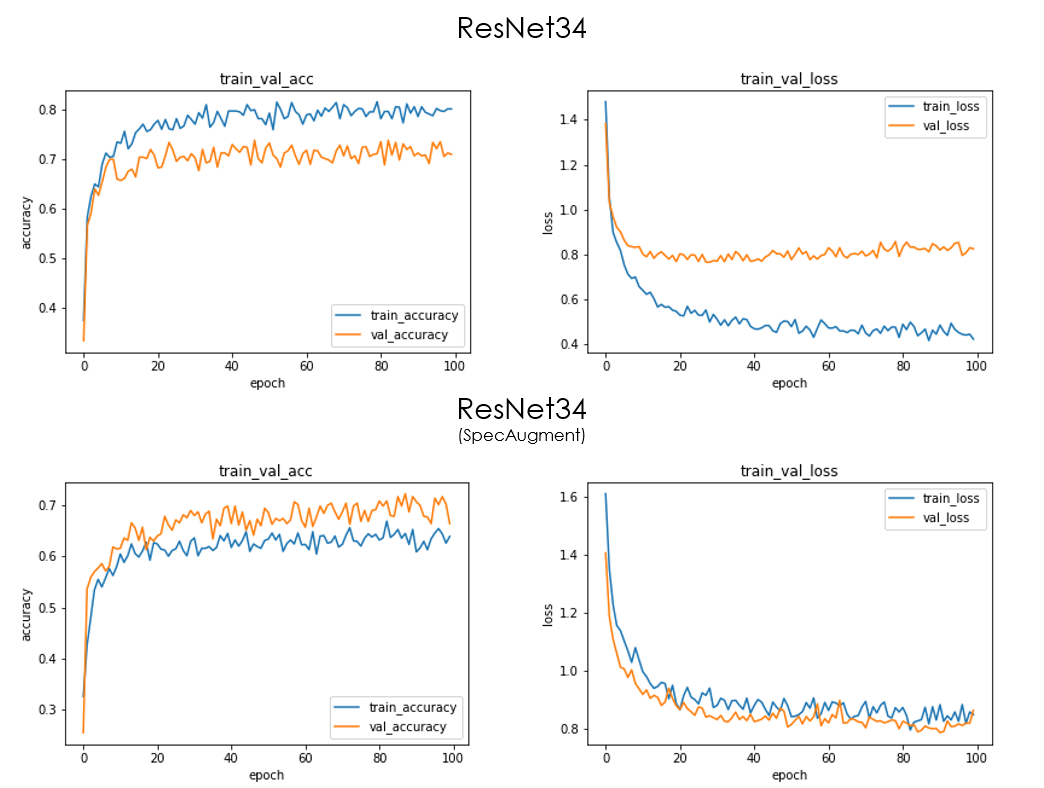
\includegraphics[scale=0.45]{resnet34_ex1.png}
  \caption{ResNet34 学習曲線 (実験 1)}
  \label{fig:resnet34_ex1}
\end{figure}

\begin{figure}[!tbh]
  \centering
  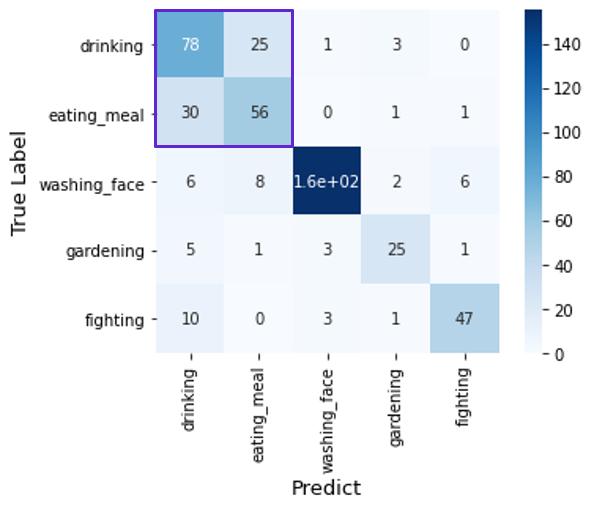
\includegraphics[scale=0.5]{ex1_cm_vgg.png}
  \caption{VGG16-BN 混合行列 (実験 1)}
  \label{fig:ex1_cm_vgg}
\end{figure}

\subsection{\small{実験 2: キャプションを入力とする動作ラベル推定}}
アノテートされたキャプションの内,「何をしているか」(action) を表すキャプションのテキストデータを JUMAN++ \cite{130007854954} によって分かち書きにしたものを, 事前学習済み Doc2Vec モデルを用いて 300 次元のベクトルに変換し, これを識別器である 3 層 MLP への入力として学習した.

表 \ref{table:caption_data_size} に実験 2 で用いたデータ数, 表 \ref{table:ex_para} に学習時のパラメータ, 表 \ref{table:d2v_para} に 事前学習済み Doc2Vec モデルのパラメータ, 表 \ref{table:mlp_para} に 3 層 MLP のパラメータを示す. 表 \ref{table:caption_data_size} において, 実験 2 では作成されたすべてのキャプションデータの内, 同じ動作ラベル内で同じ文章が 2 つ以上含まないように整形したものを用いた. 表 \ref{table:caption_data_size} より, Acc はベースラインを超えることができた. 図 \ref{fig:d2v_ex2} に学習曲線を示す. 図 \ref{fig:d2v_ex2} より, 学習曲線の推移に差が見られない事から, データの分布が大きく似ていると推測でき, これはキャプションデータがノイズの少ないデータであることに起因すると考えられる.

\begin{table}[!t]
\begin{tabular}{cc}
\begin{minipage}[c]{0.5\hsize}
\centering
\caption{学習パラメータ}
\label{table:ex_para}
\scalebox{0.7}{
\begin{tabular}{l|c}
parameter & value \\ \hline
epoch & 100 \\
batch size & 64 \\
learning rate & 0.001 \\
optimizer & Adam \\
loss function & Cross Entropy Loss
\end{tabular}
}
\end{minipage} &
\begin{minipage}[c]{0.5\hsize}
\centering
\caption{SpecAugment パラメータ}
\label{table:spec_aug_para}
\scalebox{0.7}{
\begin{tabular}{l|c}
parameter & value \\ \hline
time drop width & {[}0, 4{]} \\
time stripes num & {[}0, 1{]} \\
freq drop width & {[}0, 4{]} \\
freq stripes num & {[}0, 1{]}
\end{tabular}
}
\end{minipage}
\end {tabular}
\end{table}



\begin{table}[!t]
\begin{tabular}{cc}
\begin{minipage}[c]{0.5\hsize}
\centering
\caption{3 層 MLP パラメータ}
\label{table:mlp_para}
\scalebox{0.7}{
\begin{tabular}{l|c}
parameter & value \\ \hline
input size & 300 \\
hidden size & 30 \\
output size & 5 \\
activation function & tanh \\
dropout rate & 0.2
\end{tabular}
}
\end{minipage} &
\begin{minipage}[c]{0.5\hsize}
\centering
\caption{Doc2Vec パラメータ}
\label{table:d2v_para}
\scalebox{0.7}{
\small
\begin{tabular}{l|c}
parameter & value \\ \hline
\multirow{3}{*}{corpus} & 日本語 Wikipedia \\
 & 小説家になろう \\
 & 青空文庫 \\
vector size & 300 \\
epoch & 30 \\
window size & 8 \\
min count & 5 \\
model type & Distributed Memory
\end{tabular}
}
\end{minipage}
\end {tabular}
\end{table}



\captionsetup[table]{font=normalsize}
\captionsetup[table]{labelfont=normalsize}


\section{まとめと今後の課題}
本研究では, 最終的な目標を深層学習によるマルチメディアデータを用いた動画に対する音声の自動アノテーションを行うモデルの構築とした上で, 基礎的な実験として動画に含まれるマルチメディアデータから動画の動作を推定した. 実験結果より, データの選び方や前処理, 音声のデータ拡張方法に関して更なる模索が必要であることが分かった.
今後の課題としては以下が挙げられる.
\begin{itemize}
  \item 動画に含まれる画像データを入力とした動作ラベル推定
  \item マルチモーダルな動作ラベル推定
  \item マルチメディアデータを用いた動画に対する音声の自動アノテーションモデルの構築
\end{itemize}

\begin{figure}[!thb]
  \centering
  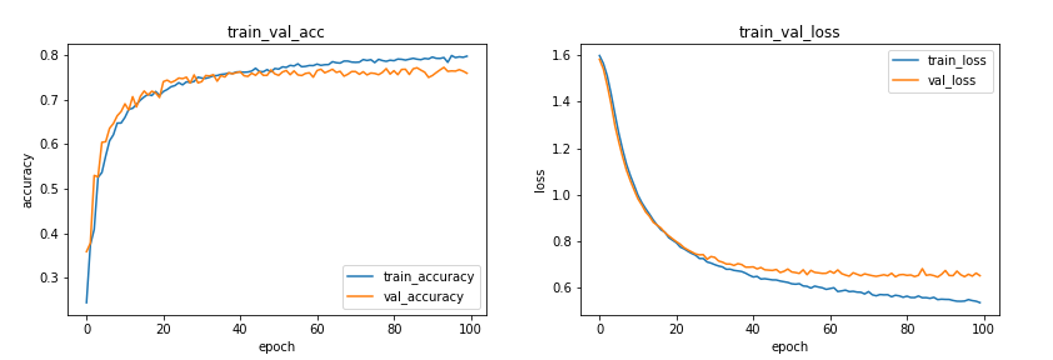
\includegraphics[scale=0.45]{d2v_ex2.png}
  \caption{学習曲線 (実験 2)}
  \label{fig:d2v_ex2}
\end{figure}


\bibliographystyle{unsrt}
\bibliography{sankou}
\end{document}
